\input{courspdf.tex}
\debutcours{Coniques}{alpha}

\section{Vocabulaire et relations}
\index{question de cours!coniques!vocabulaire et relations}
Cette section présente (\emph{sans démonstration}) les définitions et résultats à retenir.
\begin{figure}[ht]
  \hfill
  \begin{minipage}{.5\linewidth}
    \input{C4893_1.pdf_t}
    \caption{définition par foyer et directrice}
    \label{fig:C4893_1}
  \end{minipage}
  \hfill
  \begin{minipage}{.4\linewidth}
    \input{C4893_2.pdf_t}
    \caption{paramètre et axe focal}
    \label{fig:C4893_2}
  \end{minipage}
  \hfill
\end{figure}

On se donne un point noté $F$ et une droite notée $\mathcal D$ ne contenant pas $F$. Soit $M$ un point quelconque du plan, on note $H$ le projeté orthogonal de $M$ sur $\mathcal D$ (figure \ref{fig:C4893_1}). Une ligne de niveau de la fonction
\begin{displaymath}
 M \rightarrow \dfrac{d(M,F)}{d(M,\mathcal D)}
\end{displaymath}
est appelée \emph{conique}.

\subsection{Vocabulaire général}
\begin{description}
 \item[foyer] : un point $F$
\item[directrice] : une droite $\mathcal D$
\item[axe focal]\index{coniques!axe focal} : droite passant par le foyer et orthogonale à la directrice. C'est toujours un axe de symétrie.
\item[excentricité] : un réel $e$ strictement positif.
  \begin{itemize}
 \item $e<1$ : ellipse
\item  $e=1$ : parabole
\item $e>1$ : hyperbole
\end{itemize}
\item[paramètre] : \index{coniques!paramètre} nombre noté $p$ égal à la distance entre le foyer et les intersections de la courbe avec la droite parallèle à la directrice passant par le foyer. Par définition $p=e d(F,\mathcal D)$.
\item[sommets] : \index{coniques!sommet}intersection de la conique avec l'axe focal. Bien noter que, en principe, il ne faut pas appeler sommets les intersections d'une ellipse avec l'axe de symétrie qui n'est pas l'axe focal.
\end{description}

\subsection{Paramétrisation polaire : pôle à un foyer}
Le support de la courbe paramétrée
\begin{displaymath}
 \theta\rightarrow M(\theta) = F + \frac{p}{1+e\cos(\theta -\varphi)}\overrightarrow{e_\theta}
\end{displaymath}
est la conique de foyer $F$ et de directrice la droite $\mathcal{D}$ orthogonale à $\overrightarrow{u_\varphi}$ qui passe par $H_0=F+\frac{p}{e}\overrightarrow{u_\varphi}$.

\subsection{Coniques à centre: relations générales}
Il s'agit des coniques d'excentricité $e\neq 1$: les hyperboles et les ellipses.
\begin{description}
 \item[centre] : lorsque $e\neq1$ il existe un deuxième axe de symétrie. Son intersection avec l'axe focal est le centre \index{coniques!centre} noté $C$ qui est centre de symétrie de la conique.
\item[distance centre-foyer] : noté $c$.
\item[distance centre-directrice] : noté $d$.
\item[distance centre-sommet] : noté $a$.
\end{description}
Les deux formules suivantes sont valables pour les ellipses et les hyperboles
\begin{align}
  d&=\dfrac{c}{e^2} & a&=\dfrac{c}{e} \hfill
\end{align}

\subsection{Coniques à centre: relations spécifiques}
Il existe un repère orthonormé direct\footnote{en fait il en existe exactement deux} dont l'origine est au centre tel que ($x$ et $y$ désignant les fonctions coordonnées dans ce repère) l'équation cartésienne de la conique soit d'une forme particulière dite \emph{équation réduite}.
\begin{center}
\renewcommand{\arraystretch}{3}
\begin{tabular}[c]{|l|l|l|}\hline
 & ellipse & hyperbole\\ \hline
équation réduite & $\dfrac{x^2}{a^2} + \dfrac{y^2}{b^2}=1 $ & $\dfrac{x^2}{a^2} - \dfrac{y^2}{b^2}=1 $\\ \hline
condition & $0<b<a$ & $a>0$ et $b>0$ \\ \hline
distance centre-foyer $c$ & $c^2 = a^2 - b^2$ & $c^2=a^2+b^2$ \\ \hline
\end{tabular}
\end{center}
Définition bifocale. On note $F$ et $\mathcal{D}'$ les points et droite symétriques de $F$ et $\mathcal{D}$ par rapport au centre. On peut caractériser l'appartenance à la conique à l'aide des distances aux foyers.
\begin{center}
\renewcommand{\arraystretch}{3}
\begin{tabular}[c]{|l|l|}\hline
  ellipse & hyperbole\\ \hline
$FM + F'M = 2a $ & $\vert FM - F'M\vert = 2a $\\ \hline
\end{tabular}
\end{center}

\subsection{Lignes de niveau}
\begin{defi}
 Soient $a$, $b$, $c$, $d$ $e$, $f$ des réels avec $(a,b,c)\neq(0,0,0)$, soient $x$ et $y$ les fonctions coordonnées dans un repère quelconque. Une \emph{fonction du second degré} est une fonction (numérique) de la forme
\begin{displaymath}
 ax^2 + bxy +cy^2 +dx+ey+f
\end{displaymath}
Le \emph{discriminant} d'une telle fonction est le réel
\begin{displaymath}
 \Delta = b^2 -4ac
\end{displaymath}
\end{defi}
\begin{enumerate}
 \item Les coniques sont des lignes de niveau de fonctions du second degré.
 \item On étend la définition des coniques. Une ligne de niveau d'une fonction du second degré qui n'est pas une conique est appelée \emph{conique dégénérée}. Le discriminant permet de classer.
\begin{center}
\renewcommand{\arraystretch}{1.2}
\begin{tabular}{|l|l|l|}\hline
discriminant & conique & conique dégénérée\\\hline
$\Delta <0$ & ellipse & vide ou cercle\\ \hline
$\Delta =0$ & parabole & une droite ou deux droites parallèles\\ \hline
$\Delta >0$ & hyperbole & deux droites sécantes\\ \hline
\end{tabular}
\end{center}
 
\end{enumerate}



\section{\'Equation réduite}
\subsection{De la définition par foyer et directrice à l'équation réduite}
\index{question de cours!coniques!de foyer-directrice à équation réduite}
La recherche d'un deuxième axe de symétrie va nous conduire aux équations réduites.\newline
Notons $\mathcal C$ la conique de foyer $F$, de directrice $\mathcal D$ et d'excentricité $e\neq1$.\newline
On note $\delta=d(F,\mathcal D)$, $H_0$ le projeté orthogonal de $F$ sur $\mathcal D$ (intersection de la directrice et de l'axe focal ). Considérons un repère dont le premier vecteur de base (noté $\overrightarrow i$ voir figure \ref{fig:C4893_1}) est unitaire, orthogonal à la directrice et dirigé de $F$ vers $\mathcal D$ de sorte que
\begin{displaymath}
 \overrightarrow{FH_0}=\delta \overrightarrow i \text{ avec } \delta >0
\end{displaymath}
L'origine $C$ est sur l'axe focal mais n'est pas encore précisé. On choisira cette origine pour faire disparaitre le terme en $x$ dans l'équation. On note $x_F$ l'abscisse de $F$. L'équation de la directrice est alors $x=x_F+\delta$. Transformons l'équation de la conique :
\begin{multline*}
 M\in \mathcal C \Leftrightarrow FM^2 = e^2 d(M,\mathcal D)^2
 \Leftrightarrow (x-x_F)^2+y^2 = e^2(x-(x_F+\delta))^2 \\
\Leftrightarrow (1-e^2)x^2 +2\left( -x_F+e^2(x_F+\delta)\right)x+y^2 = e^2(x_F+\delta)^2 - x_F^2 
\end{multline*}
On annule le terme en $x$ en choisissant l'origine pour que
\begin{displaymath}
 -x_F+e^2(x_F+\delta) =0
\end{displaymath}
Cela devient :
\begin{displaymath}
 (1-e^2)x_F = e^2\delta \Leftrightarrow \delta = \dfrac{-e^2+1}{e^2}x_F =\left(-1+\dfrac{1}{e^2} \right)x_F 
\end{displaymath}
Ceci n'est possible que pour $e\neq 0$ d'où le nom de conique à centre pour les ellipses et les hyperboles. Il est important de remarquer que le signe de $x_F$ et les positions relatives des objets dépendent de la nature de la conique.
\begin{align*}
 x_F = \frac{e^2\delta}{1-e^2} <
x_F +\delta = x_{H_0} = \frac{\delta}{1-e^2}
\end{align*}
On en déduit les positions relatives pour la convention adoptée
\begin{center}
\renewcommand{\arraystretch}{1.2}
\begin{tabular}{|l|l|l|l|l|}\hline
genre     & excentricité & $x_F$ & $x_{H_0}$ & configuration \\ \hline
ellipse   & $<1$         & $>0$  & $>0$      & centre - foyer - directrice\\ \hline
hyperbole & $>1$         & $<0$  & $<0$      & foyer - directrice -centre\\ \hline
\end{tabular}
\end{center}
Lorsque $e$ croît vers $1$ le centre va vers l'infini sur la gauche puis revient de l'infini de l'autre côté après que $e$ ait traversé $1$. La distance centre-foyer est noté $c=|x_F|$. La distance centre-directrice est notée $d$, on obtient la première relation annoncée :
\begin{displaymath}
 d = |x_F+\delta| = \dfrac{|x_F|}{e^2}=\dfrac{c}{e^2}
\end{displaymath}
On peut alors réécrire l'équation :
\begin{align*}
 (1-e^2)x^2 + y^2 &= \dfrac{c^2}{e^2}-c^2 = \dfrac{1-e^2}{e^2}c^2 \\
\dfrac{x^2}{\frac{c^2}{e^2}} + \dfrac{y^2}{(1-e^2)\frac{c^2}{e^2}} = 1
\end{align*}
On en déduit que les sommets (intersection de la conique avec l'axe focal d'équation $y=0$) sont les points de coordonnées $(\frac{c}{e},0)$ et $(-\frac{c}{e},0)$ ce qui donne la deuxième relation annoncée.
\begin{displaymath}
 a=\frac{c}{e}
\end{displaymath}

Dans le cas d'une parabole, aucun repère ne s'impose aussi naturellement que pour les coniques à centre mais une tradition demeure. On revient à la première forme de l'équation avec $e=1$ et on développe, il vient
\begin{displaymath}
 M\in \mathcal{C}\Leftrightarrow 2\delta x + y^2 = 2\delta x_F +\delta^2 \Leftrightarrow
y^2 = 2\delta(x_F - x) + \delta^2
\end{displaymath}
On retrouve bien sous cette forme que $y=\pm \delta$ lorsque $x=x_F$ ce qui traduit $p=\delta$. Le paramètre est égal à la distance foyer-directrice. Le repère tradionnel est alors $(S,(-\overrightarrow i,-\overrightarrow j))$. Si $X$ et $Y$ sont les fonctions coordonnées dans ce repère l'équation devient
\begin{displaymath}
 Y^2 = 2pX
\end{displaymath}


\subsection{Conséquences de l'équation réduite}\index{coniques!équation réduite}
\begin{figure}[ht]
  \hfill
  \begin{minipage}{.45\linewidth}
    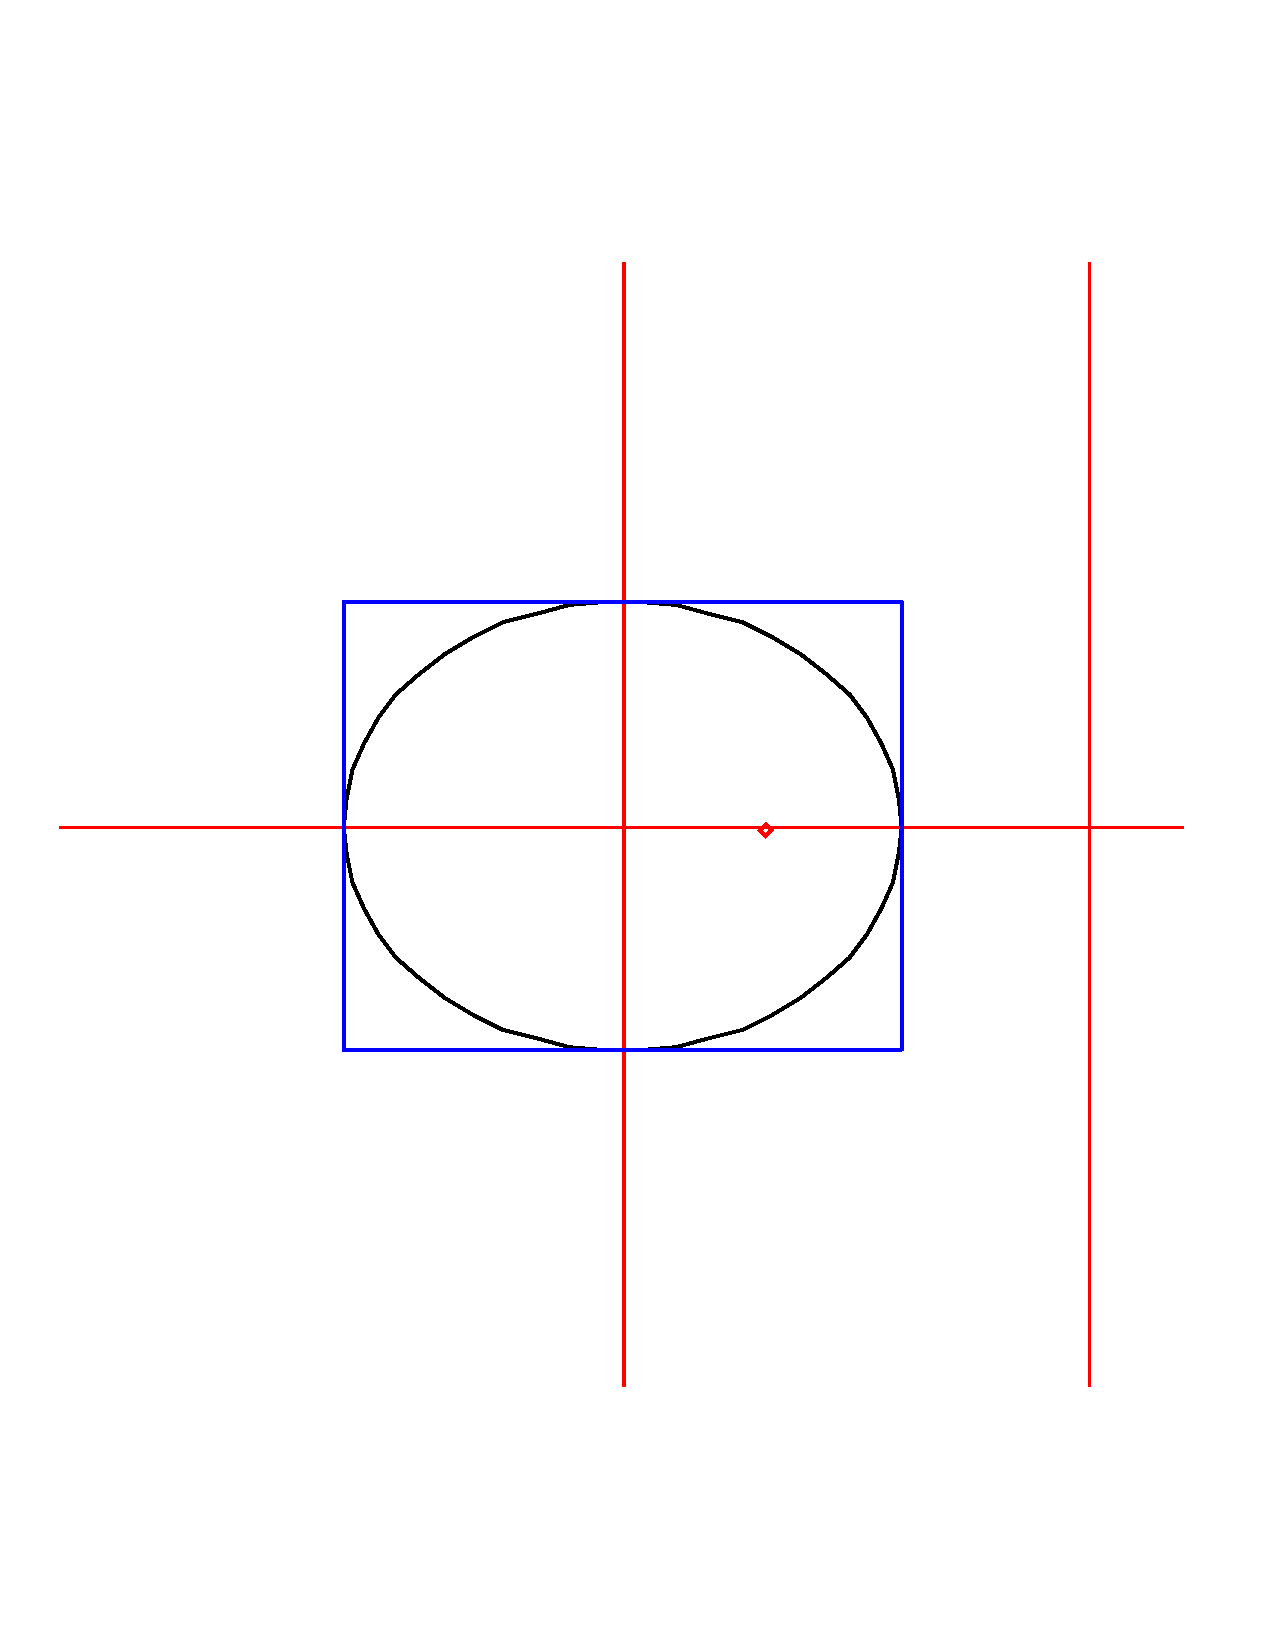
\includegraphics[width=7.5cm]{C4893_3.pdf}
    \caption{ellipse}
    \label{fig:C4893_3}
  \end{minipage}
  \hfill
  \begin{minipage}{.45\linewidth}
    \includegraphics[width=7.5cm]{C4893_4.pdf}
    \caption{hyperbole}
    \label{fig:C4893_4}
  \end{minipage}
  \hfill
\end{figure}

\`A la fin du paragraphe précédent nous sommes arrivés (pour une conique $\mathcal C$ d'excentricité différente de $1$) à une équation de la forme
\begin{displaymath}
\dfrac{x^2}{\frac{c^2}{e^2}} + \dfrac{y^2}{(1-e^2)\frac{c^2}{e^2}} = 1
\end{displaymath}
Cette formule prend une forme différente suivant que $e$ est plus petit ou plus grand que 1.
\subsubsection{Ellipse}
\begin{displaymath}
\dfrac{x^2}{a^2} + \dfrac{y^2}{b^2} = 1
\end{displaymath}
avec 
\begin{align*}
 a &= \dfrac{c}{e} & b^2 &= (1-e^2)\dfrac{c^2}{e^2}=a^2 - c^2 & 0<b<c
\end{align*}
On en déduit diverses propriétés :
\begin{itemize}
 \item L'ellipse est incluse dans un rectangle : si $M\in \mathcal C$ alors $|x(M)|\leq a$ et $|y(M)|\leq b$.
\item Comme $d=\frac{c}{e^2}=\frac{a}{e}>a$, les directrices sont à l'extérieur de ce rectangle.
\item la fonction $t \rightarrow O +a\cos t \overrightarrow{i} + b\sin t \overrightarrow{j}$ est une paramétrisation de $\mathcal C$.
\item L'ellipse $\mathcal C$ est l'image du cercle de centre $O$ et de rayon $a$ par l'affinité orthogonale d'axe $Ox$ et de rapport $\frac{b}{a}$\index{affinité orthogonale}\index{cercle principal} c'est à dire l`application 
\begin{displaymath}
 M \rightarrow O +x(M)\overrightarrow{i} + \dfrac{b}{a}y(M)\overrightarrow{j}
\end{displaymath}
Construction géométrique avec les cercles de rayon $a$ et $b$.
\end{itemize}

\subsubsection{Hyperbole}
\begin{displaymath}
\dfrac{x^2}{a^2} - \dfrac{y^2}{b^2} = 1
\end{displaymath}
avec 
\begin{align*}
 a&>0 & b&>0 & a &= \dfrac{c}{e} & b^2 &= (e^2-1)\dfrac{c^2}{e^2}=c^2 - a^2
\end{align*}
On en déduit diverses propriétés :
\begin{itemize}
 \item L'hyperbole est en dehors d'une bande verticale : si $M\in \mathcal C$ alors $|x(M)|\leq a$.
\item Comme $d=\frac{c}{e^2}=\frac{a}{e}<a$, les directrices sont dans cette bande.
\item la fonction $t \rightarrow O +a\ch t \overrightarrow{i} + b\sh t \overrightarrow{j}$ est une paramétrisation de $\mathcal C$.
\item La paramétrisation précédente permet de montrer que les droites d'équation
\begin{align*}
 \dfrac{x}{a}+\dfrac{y}{b}&=0 & \dfrac{x}{a}-\dfrac{y}{b}&= 0
\end{align*}
sont asymptotes
\item hyperbole équilatère\index{hyperbole équilatère}, repère attaché aux asymptotes
\end{itemize}
\subsubsection{Parabole}
\begin{figure}[h!]
 \centering
 \includegraphics{./C4893_9.pdf}
 % C4893_9.pdf: 292x243 pixel, 72dpi, 10.30x8.57 cm, bb=0 0 292 243
 \caption{parabole}
 \label{fig:C4893_9}
\end{figure}
On considère une parabole d'équation 
\begin{displaymath}
 y^2 = 2p x
\end{displaymath}
On peut en déduire diverse propriétés
\begin{itemize}
 \item Si $M$ est sur la parabole $x(M)\geq 0$.
 \item L'origine est au sommet. Distance - foyer directrice = $p$. Distance sommet-foyer=$\frac{p}{2}$.
 \item On peut paramétrer par $y$ :
\begin{displaymath}
 t\rightarrow O + \frac{t^2}{2p}\overrightarrow i + t\,\overrightarrow j
\end{displaymath}

\end{itemize}



\section{Définition bifocale}
\subsection{Régionnement et directrices}
\begin{figure}[ht]
  \hfill
  \begin{minipage}{.45\linewidth}
    \input{C4893_5.pdf_t}
    \caption{ellipse : $d=\dfrac{a}{e}>a$}
    \label{fig:C4893_5}
  \end{minipage}
  \hfill
  \begin{minipage}{.45\linewidth}
    \input{C4893_6.pdf_t}
    \caption{hyperbole : $d=\dfrac{a}{e}<a$}
    \label{fig:C4893_6}
  \end{minipage}
  \hfill
\end{figure}
Considérons d'abord quelques objets et formules valables pour les deux types de conique à centre à partir de la donnée d'un foyer, d'une directrice et d'une excentricité. Notons en particulier $\mathcal C$ la conique définie par ces données.
\begin{align*}
 \text{distance centre-sommet} : a &=\dfrac{c}{e}\\ \\
 \text{distance centre-directrice} : d &=\dfrac{c}{e^2}=\dfrac{a}{e}
\end{align*}
La différence des carrés des distances aux foyers s'exprime aussi de la même manière:
\begin{align*}
 MF^2 = (x(M)-c)^2+y(M)^2 & & MF'^2 = (x(M)+c)^2+y(M)^2 
\end{align*}
on en déduit :
\begin{displaymath}
  MF^2 - MF'^2 = -4x(M)c = (MF + MF')(MF - MF')
\end{displaymath}

On peut auusi écrire
\begin{align*}
 ed(M,\mathcal D)= e|x(M)-d| = |ex(M)-a| & &
 ed(M,\mathcal D')= e|x(M)+d| = |ex(M)+a| 
\end{align*}
Introduisons alors trois parties du plan définies par les directrices.
\begin{center}
\renewcommand{\arraystretch}{1.5}
% use packages: array
\begin{tabular}{c|c|c|c|c}
partie & description & caractérisation  & $ed(M,\mathcal D)$ & $ed(M,\mathcal D')$ \\ \hline
$M\in \mathcal P_+$ & $M$ à droite de $\mathcal D$ & $x(M)>d$ & $ex(M)-a$ & $ex(M)+a$ \\ \hline
$M\in \mathcal P_-$ & $M$ à gauche de $\mathcal D'$ & $x(M)<-d$ & $-ex(M)+a$ & $-ex(M)-a$ \\ \hline
$M\in \mathcal P_0$ & $M$ entre $\mathcal D'$ et $\mathcal D$& $-d<x(M)<d$ &  $-ex(M)+a$  &  $ex(M)+a$
\end{tabular}
\end{center}
\subsection{De la définition par foyer et directrice vers la définition bifocale}\index{question de cours!coniques!définition bifocale}
Dans le cas où $e<1$, la conique $\mathcal C$ est une ellipse. L'étude des équations réduites a montré que $\mathcal C \subset \mathcal P_0$. Le tableau entraine alors :
\begin{displaymath}
 M\in \mathcal C \Rightarrow MF + MF' = ed(M,\mathcal D) + ed(M,\mathcal D') = 2a
\end{displaymath}
Dans le cas où $e>1$, la conique  $\mathcal C$ est une hyperbole. L'étude des équations réduites à montré qu'elle est constituée de deux branches : $\mathcal C = \mathcal H_+ \cup \mathcal H_+$ telles que $\mathcal H_+\subset P_+$ et $\mathcal H_-\subset P_-$. Le tableau entraîne alors :
\begin{align*}
 M\in \mathcal H_+ &\Rightarrow MF - MF' = ed(M,\mathcal D) + ed(M,\mathcal D') = -2a \\
 M\in \mathcal H_- &\Rightarrow MF - MF' = ed(M,\mathcal D) + ed(M,\mathcal D') = 2a \\
\end{align*}

\subsection{De la définition bifocale vers la définition par foyer et directrice}
On se donne deux points $F$ et $F'$ de coordonnées $(c,0)$ et $(-c,0)$ et un réel $a>0$. On pose :
\begin{align*}
 e=\dfrac{c}{a} & & d=\dfrac{a}{e} & & \mathcal D : \text{droite d'eq }x=d & & \mathcal D' : \text{droite d'eq }x=-d
\end{align*}
On définit aussi les points $S$ et $S'$ de coordonnées $(a,0)$ et $(-a,0)$ et la conique $\mathcal C$ définie par ces données. On peut alors utiliser les objets et formules définies au début. 
\begin{figure}[ht]
  \hfill
  \begin{minipage}{.45\linewidth}
    \input{C4893_7.pdf_t}
    \caption{$a>c , e<1 , d>a$}
    \label{fig:C4893_7}
  \end{minipage}
  \hfill
  \begin{minipage}{.45\linewidth}
    \input{C4893_8.pdf_t}
    \caption{$a<c , e>1 , d<a$}
    \label{fig:C4893_8}
  \end{minipage}
  \hfill
\end{figure}
\begin{itemize}
 \item Si $a>c$ et $M$ un point du plan tel que $MF+MF'=2a$. Alors
\begin{displaymath}
  MF^2 - MF'^2 = -4x(M)c = (MF + MF')(MF - MF') \Rightarrow
MF - MF' = -2\dfrac{c}{a}x(M)= -2ex(M)
\end{displaymath}
puis
\begin{displaymath}
 \left. 
\begin{aligned}
 MF+MF'&=2a \\
MF - MF' &= -2ex(M)
\end{aligned}
\right\rbrace \Rightarrow
MF = a-ex(M) = e(d-x(M))
\end{displaymath}
Ceci entraîne que $d-x(M)$ est positif et égal à $d(M,\mathcal D)$. On en déduit $MF=ed(M,\mathcal D)$.\newline
Le point est donc sur l'ellipse.

\item Si $a>c$ et $M$ un point du plan tel que $MF-MF'=2a$. Alors
\begin{displaymath}
  MF^2 - MF'^2 = -4x(M)c = (MF + MF')(MF - MF') \Rightarrow
MF + MF' = -2\dfrac{c}{a}x(M)= -2ex(M)
\end{displaymath}
puis
\begin{displaymath}
 \left. 
\begin{aligned}
 MF-MF'&=2a \\
MF + MF' &= -2ex(M)
\end{aligned}
\right\rbrace \Rightarrow
MF = a-ex(M) = e(d-x(M))
\end{displaymath}
Ceci entraîne que $d-x(M)$ est positif (donc $M \notin \mathcal P_+$ et égal à $d(M,\mathcal D)$. On en déduit $MF=ed(M,\mathcal D)$.\\
Le point est donc sur l'hyperbole, plus précisément sur la branche $\mathcal H_-$ car il n'est pas dans $\mathcal P_+$.

\item Si $a>c$ et $M$ un point du plan tel que $MF-MF'=-2a$. Alors
\begin{displaymath}
  MF^2 - MF'^2 = -4x(M)c = (MF + MF')(MF - MF') \Rightarrow
MF + MF' = 2\dfrac{c}{a}x(M)= 2ex(M)
\end{displaymath}
puis
\begin{displaymath}
 \left. 
\begin{aligned}
 MF-MF'&= -2a \\
MF + MF' &= 2ex(M)
\end{aligned}
\right\rbrace \Rightarrow
MF = -a+ex(M) = e(-d+x(M))
\end{displaymath}
Ceci entraîne que $-d+x(M)$ est positif (donc $M\in \mathcal P_+$ et égal à $d(M,\mathcal D)$. On en déduit $MF=ed(M,\mathcal D)$. Il est donc sur la conique, plus précisément sur la branche $\mathcal H_+$.
\end{itemize}
\begin{rem}[éléments à partir d'une définition bifocale]
 \index{savoir-faire!coniques!éléments à partir d'une définition bifocale}
On peut utiliser cette démonstration pour déterminer pratiquement les éléments d'une conique définie à partir de ses deux foyers. Par exemple soit $F$ et $F'$ tels que $FF'=6$ et  $\mathcal{E}$ la conique définie par :
\begin{displaymath}
 M\in \mathcal{C} \Leftrightarrow FM + F'M = 10
\end{displaymath}
 On choisit un repère dont l'origine est au milieu des foyers, l'axe $Ox$ est l'axe focal dirigé de $F$ vers $F'$ de sorte que les coordonnées de $F$ sont $(3,0)$ et celles de $F'$ sont $(-3,0)$ avec $c=3$ et $a=5$. Alors
\begin{displaymath}
\left. 
\begin{aligned}
FM^2 - F'M^2 &= (x-3)^2 - (x+3)^2 = -12x \\
FM + F'M &= 10
\end{aligned}
\right\rbrace \Rightarrow
\left. 
\begin{aligned}
FM - F'M &= -\frac{6}{5}x \\
FM + F'M &= 10
\end{aligned}
\right\rbrace \Rightarrow
FM = -\frac{3}{5}x+5 = \frac{3}{5}\left( \frac{25}{3}-x\right)  
\end{displaymath}
On en déduit l'excentricité 
\begin{displaymath}
 e=\frac{3}{5}
\end{displaymath}
\end{rem}



\section{Lignes de niveau d'une fonction numérique du second degré}
\subsection{Discriminant}
Discriminant et déterminant du système de recherche du centre
\index{savoir-faire!coniques!recherche du centre}
\subsection{Recherche d'une équation réduite}
\index{changement de repère}\index{savoir-faire!coniques!élimination du terme en $xy$}
Exemple pour $f = x^2 + xy +y^2 -2$.
On définit un nouveau système de coordonnées :
\begin{displaymath}
\begin{aligned}
 x &= \cos (\theta)\, X + \sin(\theta)\, Y \\
 y &= -\sin (\theta)\, X +\cos (\theta)\, Y
\end{aligned} 
\end{displaymath}
et on cherche les $\theta$ annulant le terme en $XY$ en remplaçant dans l'expression. Si on ne dispose pas d'un logiciel de calcul formel, il est commode de procéder en tableau:
\begin{multline*}
 \left.
\begin{aligned}
 x^2 &= \cos^2 (\theta)\, X^2 + \sin^2(\theta)\, Y^2 + 2 \sin(\theta)\, \cos (\theta)\, XY \\ 
 y^2 &= \sin^2 (\theta)\, X^2 + \cos^2 (\theta)\, Y^2-+ 2 \sin(\theta)\, \cos (\theta)\, XY\\
 xy &= -\cos (\theta)\, \sin (\theta)\, X^2+\cos (\theta)\, \sin (\theta)\, Y^2 +(\cos^2(\theta)\, -\sin^2(\theta)\,)XY
\end{aligned}
 \right\rbrace 
\Rightarrow \\
\text{ terme $XY$ de $f =$ } \cos^2(\theta)\, -\sin^2(\theta)=\cos(2\theta)
\end{multline*}
On choisit alors $\theta=\frac{\pi}{4}$ et on remplace. (cela ne sera pas forcément le choix définitif)
\begin{displaymath}
 f = \frac{1}{2}X^2 - \frac{3}{2}Y^2 -2
\end{displaymath}
puis 
\begin{displaymath}
 \frac{1}{2}X^2 - \frac{3}{2}Y^2 -2 = 0
\Leftrightarrow
\frac{X^2}{4}+\frac{Y^2}{\frac{4}{3}} = 1
\end{displaymath}
Ceci est bien une équation réduite (d'une ellipse) avec $a=2>b=\frac{2}{\sqrt{3}}$. Dans certains cas il faut permuter les deux axes pour bien avoir l'axe focal comme axe $Ox$.
\subsection{Tangente}
\index{question de cours!règle du dédoublement}Règle du dédoublement
\subsection{Coniques passant par des points donnés}
\section{Paramétrisations}
\subsection{Paramétrisation trigonométrique : origine au centre}
\begin{displaymath}
 t \rightarrow C + a\cos t \overrightarrow i + b\sin t \overrightarrow j 
\end{displaymath}
\begin{displaymath}
 t \rightarrow C + a\ch t \overrightarrow i + b\sh t \overrightarrow j.
\end{displaymath}
à rédiger

il s'agit de courbes paramétrées à accélération centrale\index{courbe paramétrée à accélération centrale}. Le paramètre $t$ est proportionnel à l'aire balayée (cercle principal)
\index{question de cours!coniques!paramétrisation polaire}
\subsection{Paramétrisation polaire : pôle à un foyer}
\begin{displaymath}
 \theta\rightarrow M(\theta) = F + \frac{p}{1+e\cos(\theta -\varphi)}\overrightarrow{e_\theta}
\end{displaymath}
Définissons le point $H_0 = F + \frac{p}{e}\overrightarrow{u_\varphi}$ et la droite $\mathcal D$ passant par $H_0$ et orthogonale à $\overrightarrow{u_\varphi}$. Calculons alors
\begin{displaymath}
 (\overrightarrow{H_0M(\theta)}/\overrightarrow{u_\varphi})
\end{displaymath}
dont la valeur absolue est la distance de $M(\theta)$ à $\mathcal D$. Comme 
\begin{displaymath}
 \overrightarrow{H_0M(\theta)} = \overrightarrow{H_0F} + \overrightarrow{FM(\theta)}=
-\frac{p}{e}\overrightarrow{u_\theta}+ \overrightarrow{FM(\theta)}
\end{displaymath}
il vient :
\begin{displaymath}
 (\overrightarrow{H_0M(\theta)}/\overrightarrow{u_\varphi})=
-\frac{p}{e}+ \frac{p}{1+e\cos(\theta -\varphi)}\cos(\theta -\varphi)= \frac{p}{1+e\cos(\theta -\varphi)}
\end{displaymath}
On en déduit que
\begin{displaymath}
 d(M(\theta),\mathcal D) = \vert (\overrightarrow{H_0M(\theta)}/\overrightarrow{u_\varphi})\vert
= \frac{1}{e}OM(\theta)
\end{displaymath}
Ce qui prouve bien que $M(\theta)$ est sur la conique de foyer $F$ de directrice $\mathcal D$ et d'excentricité $e$.
\begin{rem}
 Dans le cas d'une hyperbole ($e>1$), le réel
\begin{displaymath}
 r(\theta) = \frac{p}{1+e\cos(\theta -\varphi)}
\end{displaymath}
n'est pas toujours strictement positif. L'annulation du dénominateur correspond aux asymptotes ... à rédiger
\end{rem}

\subsection{Paramétrisation rationnelle}
On fixe un point $M_0$ de la conique et on considère les droites qui passent par ce point. Elles coupent la conique en deux points dont $M_0$. On peut donc associer un point de la conique à chaque droite. Si par exemple on note $D_t$ la droite qui passe par $M_0$ et de direction $\overrightarrow i + t\overrightarrow j$, on obtient ainsi une paramétrisation de la conique éventuellement privée du point $M_0$.
\end{document}
